\documentclass[12pt]{article}
\usepackage[pdftex]{graphicx}
\usepackage[utf8x]{inputenc}
\usepackage[left=1.5cm,right=1.5cm,top=1.5cm,bottom=1.5cm]{geometry}
\usepackage[russian]{babel}
\DeclareGraphicsExtensions{.pdf,.png,.jpg}
\title{Cкорость считывания}  
\date{08/09/2016}  
\author{Kailiak Eugene}

\begin{document}
\maketitle
Числа типа double генерировались c помощью указанной ниже программы на Python 3.4\\
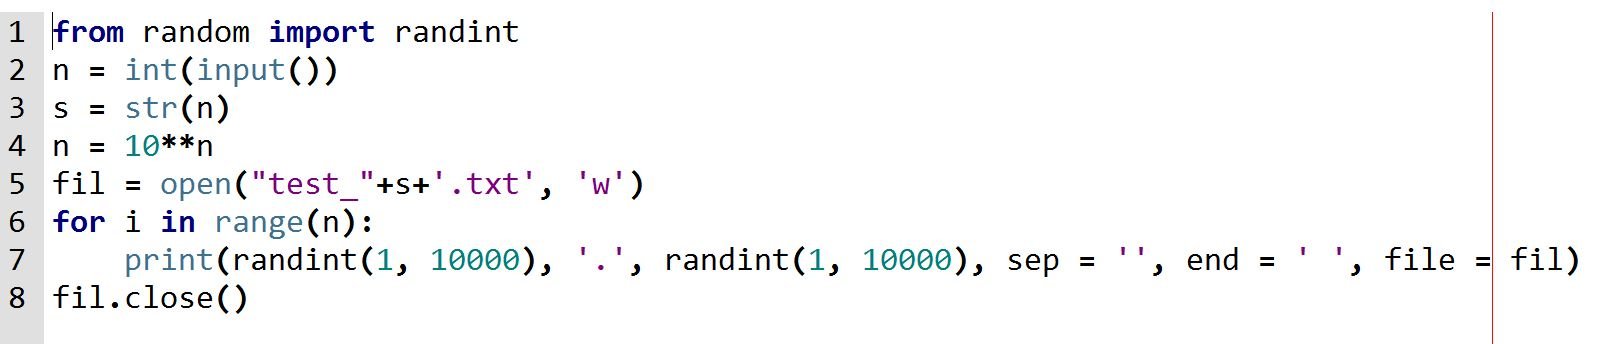
\includegraphics{make_test} \\

Для того, чтобы сравнить скорость считывания scanf и std::cin, я использовал следующую программу: \\
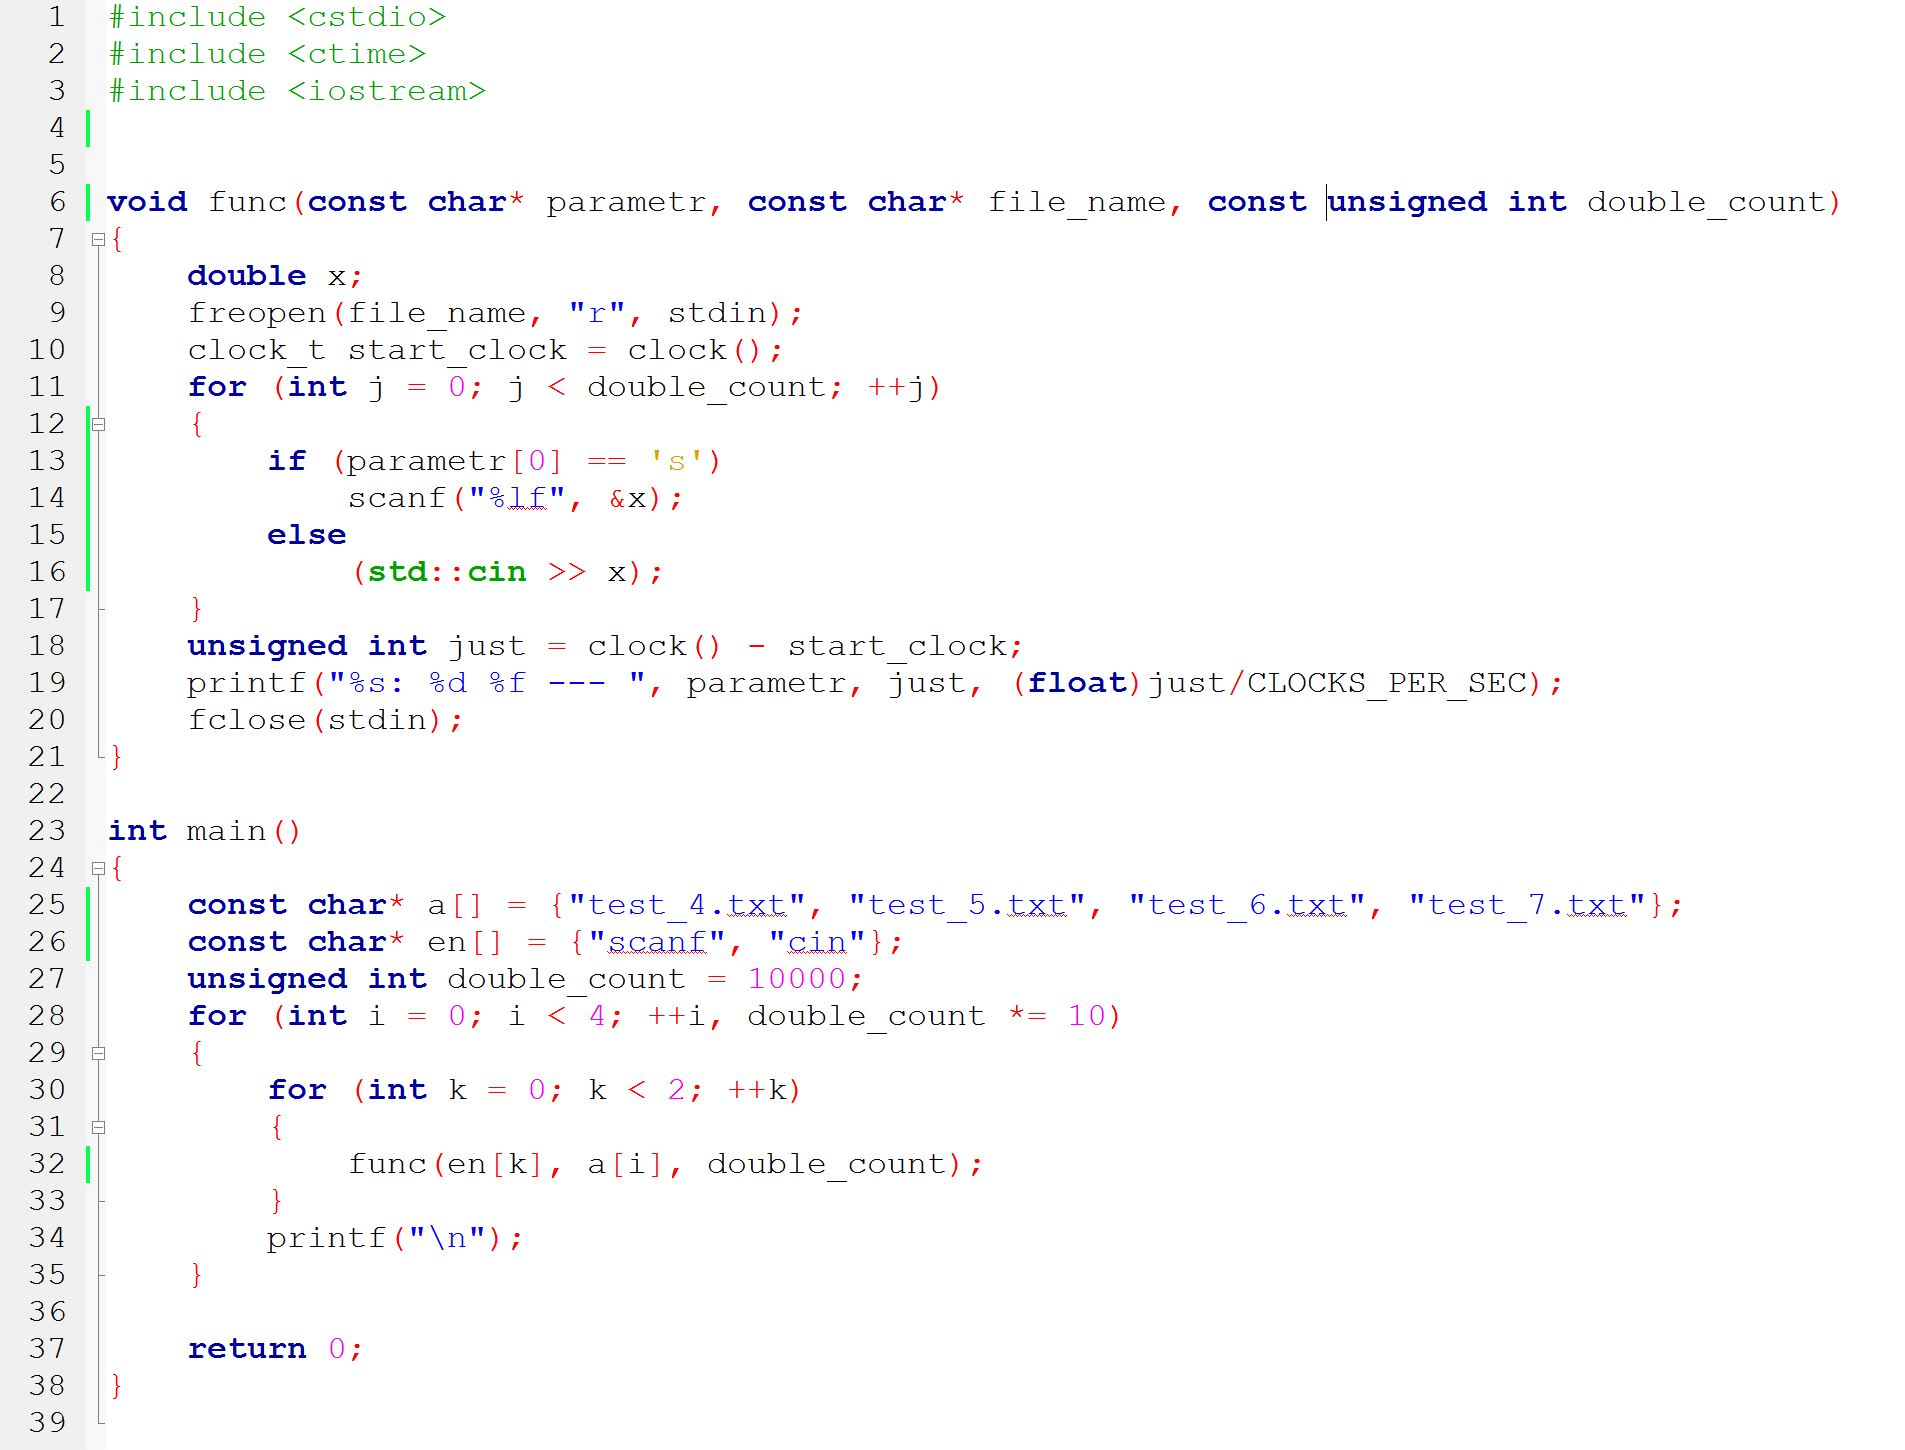
\includegraphics[width=18cm]{Programm} \\

Где по порядку открываются файлы $test\_n.txt, n = 4,5,6,7$ Файл содержит $10^n$ чисел типа double \\
Вот результат работы программы, где первое число - число тактов, второе - число секунд. Количество числе типа double различается построчно, увеличивается с каждой строчкой. \\
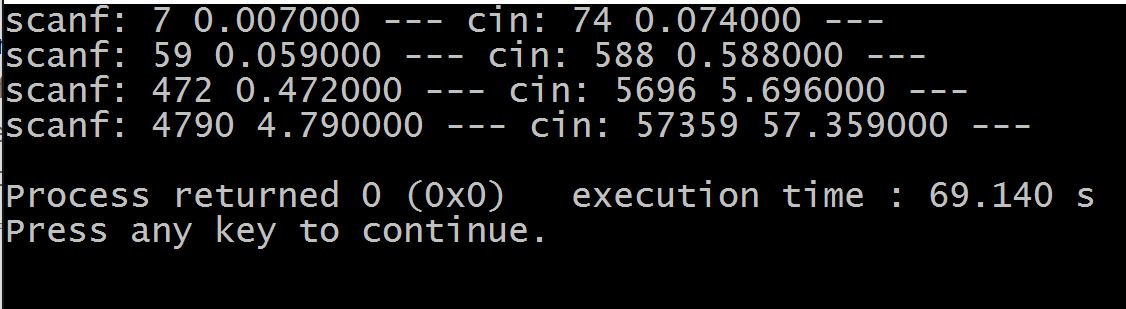
\includegraphics{Results} \\
Получается, что scanf сильно быстрее, чем std::cin. На каждом количестве тестов скорость считывания scanf на порядок больше std::cin \\
\end{document}